\documentclass[a4paper]{extarticle}
\usepackage[utf8]{inputenc}
\usepackage[a4paper, margin=1in]{geometry}

\usepackage{amssymb}
\usepackage{amsmath}
\usepackage{enumitem}
\usepackage{tcolorbox}
\usepackage{fancyhdr}
\usepackage{graphicx}
\usepackage{float}
\usepackage{bbm}

\setlength{\parindent}{0em}
\setlength{\parskip}{0.4em}

\definecolor{theoremblue}{RGB}{1, 73, 124}
\definecolor{corollaryblue}{RGB}{70, 143, 175}
\definecolor{exampleblue}{RGB}{137, 194, 217}

\newtcolorbox{tbox}{colback=theoremblue!20,colframe=theoremblue,
boxrule=0pt,arc=0pt,boxsep=2pt,left=2pt,right=2pt,leftrule=2pt}

\newtcolorbox{cbox}{colback=corollaryblue!20,colframe=corollaryblue,
boxrule=0pt,arc=0pt,boxsep=2pt,left=2pt,right=2pt,leftrule=2pt}

\newtcolorbox{ebox}{colback=exampleblue!20,colframe=exampleblue,
boxrule=0pt,arc=0pt,boxsep=2pt,left=2pt,right=2pt,leftrule=2pt}

\title{WuS - Lecture Notes Week 3}
\author{Ruben Schenk, ruben.schenk@inf.ethz.ch}
\date{\today}

\pagestyle{fancy}
\fancyhf{}
\rhead{ruben.schenk@inf.ethz.ch}
\rfoot{Page \thepage}
\lhead{WuS - Lecture Notes Week 3}

\begin{document}

\maketitle

\section{Random Variables and Distribution Functions}

\subsection{Abstract Definition}

\textbf{Definition:} Let \((\Omega, \, \mathcal{F}, \, \mathbb{P})\) be a probability space. A \textbf{random variable (r.v.)} is a map \(X : \Omega \to \mathbb{R}\) such that for all \(a \in \mathbb{R}\),
\[
    \{\omega \in \Omega : X(\omega) \leq a\} \in \mathcal{F}.
\]
The condition \(\{\omega \in \Omega : X(\omega) \leq a\} \in \mathcal{F}\) is needed for \(\mathbb{P}[\{w \in \Omega : X(\omega) \leq a\}]\) to be well-defined.

\begin{ebox}
    \textbf{Example (Indicator function of an event):} Let \(A \in \mathcal{F}\). Consider the \textbf{indicator function} \(\mathbbm{1}_A\) of \(A\), defined by
    \[
        \forall \omega \in \Omega : X(\omega) = \begin{cases}
            0 \quad &\text{if } \omega \notin A, \\
            1 \quad &\text{if } \omega \in A.
        \end{cases}
    \]
    Then \(\mathbbm{1}_A\) is a random variable. Indeed, we have
    \[
        \{\omega : \mathbbm{1}_A(\omega) \leq a\} = \begin{cases}
            \emptyset \quad &\text{if } a < 0, \\
            A^C \quad &\text{if } 0 \leq a \leq 1, \\
            \Omega \quad &\text{if } a \geq 1,
        \end{cases}
    \]
    and \(\emptyset, \, A^C,\) and \(\Omega\) are three elements of \(\mathcal{F}\).
\end{ebox}

\textbf{Notation:} When events are defined in terms of random variables, we will \textit{omit the dependence in} \(\omega\). For example, for \(a \leq b\) we write:
\begin{align*}
    &\{X \leq a\} = \{\omega \in \Omega : X(\omega) \leq a\},\\
    &\{a < X \leq b\} = \{\omega \in \Omega : a X(\omega) < b\},\\
    &\{X \in \mathbb{Z}\} = \{\omega \in \Omega : X(\omega) \in \mathbb{Z}\}
\end{align*}
When considering the probability of the events above, we omit the brackets and, for example, simply write:
\[
    \mathbb{P}[X \leq a] = \mathbb{P}[\{X \leq a\}] = \mathbb{P}[\{\omega \in \Omega : X(\omega) \leq a\}].
\]

\subsection{Distribution Function}

\textbf{Definition:} Let \(X\) be a random variable on a probability space \((\Omega, \, \mathcal{F}, \, \mathbb{P})\). The \textbf{distribution function} of \(X\) is the function \(F_X : \mathbb{R} \to [0, \, 1]\) defined by
\[
    \forall a \in \mathbb{R} : F_X(a) = \mathbb{P}[X \leq a]
\]
The idead is that the distribution function \(F_X\) encodes the probabilistic properties of the random variable \(X\).

\begin{tbox}
    \textbf{Proposition (Basic identity):} Let \(a < b\) be two real numbers. Then
    \[
        \mathbb{P}[a < X \leq b] = F(b) - F(a)
    \]
\end{tbox}

\begin{tbox}
    \textbf{Theorem (Properties of distribution functions):} Let \(X\) be a random variable on some probability space \((\Omega, \, \mathcal{F}), \, \mathbb{P}\). The distribution function \(F = F_X : \mathbb{R} \to [0, \, 1]\) of \(X\) satisfies the following properties:
    \begin{enumerate}
        \item \(F\) is nondecreasing.
        \item \(F\) is right continuous, i.e. \(F(a) = \lim_{h \downarrow 0}F(a + h)\) for every \(a \in \mathbb{R}\).
        \item \(\lim_{a \to - \infty} F(a) = 0\) and \(\lim_{a \to \infty} F(a) = 1\).
    \end{enumerate}
\end{tbox}

\subsection{Independence}

\subsubsection{Independence of Random Variables}

\textbf{Definition:} Let \(X_1,..., \, X_n\) be \(n\) random variables on some probability space \((\Omega, \, \mathcal{F}, \, \mathbb{P})\). We say that \(X_1,..., \, X_n\) are \textbf{independent} if
\[
    \forall x_1,..., \, x_n \in \mathbb{R} : \mathbb{P}[X_1 \leq x_1,..., \, X_n \leq x_n] = \mathbb{P}[X_1 \leq x_1] \cdots \mathbb{P}[X_n \leq x_n].
\]

\textbf{Definition:} An infinite sequence \(X_1, \, X_2,...\) of random variables is said to be:

\begin{itemize}
    \item \textbf{independent} ix \(X_1,..., \, X_n\) are independent, for every \(n\).
    \item \textbf{independent and identically distributed (iid)} if they are independent and have the same distribution function, i.e. \(\forall i, \, y : F_{X_i} = F_{X_j}\).
\end{itemize}

\subsection{Transformation of Random Variables}

Once we have some random variables \(X_1, \, X_2,...\) on some probability space \((\Omega, \, \mathcal{F}, \, \mathbb{P})\), we can create and consider many new random variables on the same probability space by using operations. For example, one can consider \(Z_1 = X_1 + X_2\). However, one should not forget that random variables are maps \(\Omega \to \mathbb{R}\). For example, the random variable \(Z_1\) corresponds to the map, defined for every \(\omega \in \Omega\), \(Z_1(\omega) = X_1(\omega) + X_2(\omega)\).

Formally, we introduce the following notation, which allows us to work with random variables as if they were just real numbers. If \(X\) is the random variable, and \(\phi : \mathbb{R} \to \mathbb{R}\), then we write
\[
    \phi(X) := \phi \circ X.
\]
This way, \(\phi(X)\) is a new mapping \(\Omega \to \mathbb{R}\) as show in the following diagram:
\begin{align*}
    &\Omega \to^{X} \mathbb{R} \to^{\phi} \mathbb{R} \\
    &\omega \to X(\omega) \to \phi(X(\omega)).
\end{align*}

\subsection{Construction of Random Variables}

The goal of this section is to construct general random variables. Our approach will rely on the abstract theorem of Kolmogorov, that guarantees existences of iid sequences. The construction proceeds in 4 steps:

\paragraph{Step 1: Komogorov theorem and iid sequence of Bernoulli random variables}
Our construction starts with Bernoulli random variables, that we define now.

\textbf{Definition:} Let \(p \in [0, \, 1]\). A random variable \(X\) is said to be a \textbf{Bernoulli random variable with parameter} \(p\) if
\[
    \mathbb{P}[X = 0] = 1 - p \text{ and } \mathbb{P}[X = 1] = p.
\]
In this case, we write \(X \sim \text{Ber}(p)\).

\begin{tbox}
    \textbf{Theorem (Existence theorem of Kolmogorov):} There exists a probability space \((\Omega, \, \mathcal{F}, \, \mathbb{P})\) and an infinite sequence of random variables \(X_1, \, X_2,...\) (on this probability space) that is an iid sequence of Bernoulli random variables with parameter \(\frac{1}{2}\).
\end{tbox}

\paragraph{Step 2: Construction of a uniform random variable in \([0, \, 1]\)}
Here we use Bernoulli random variables to construct a uniform random variable in \([0, \, 1]\). Intuitively, one can imagine a droplet of water falling in the interval \([0, \, 1]\). A uniform random variable in \([0, \, 1]\) represents the position at which such a droplet falls.

\textbf{Definition:} A random variable \(U\) is said to be a \textbf{uniform random variable in} \([0, \, 1]\) if its distribution function is equal to
\[
    F_U(x) = \begin{cases}
        0, &x < 0, \\
        x, &0 \leq x \leq 1, \\
        1, &x > 1.
    \end{cases}
\]
In this case, we write \(U \sim \mathcal{U}([0, \, 1])\).

The figure below shows the distribution function of a Bernoulli r.v. with parameter \(p\) (left) and the distribution function of a uniform random variable in \([0, \, 1]\) (right).

\begin{figure}[H]
    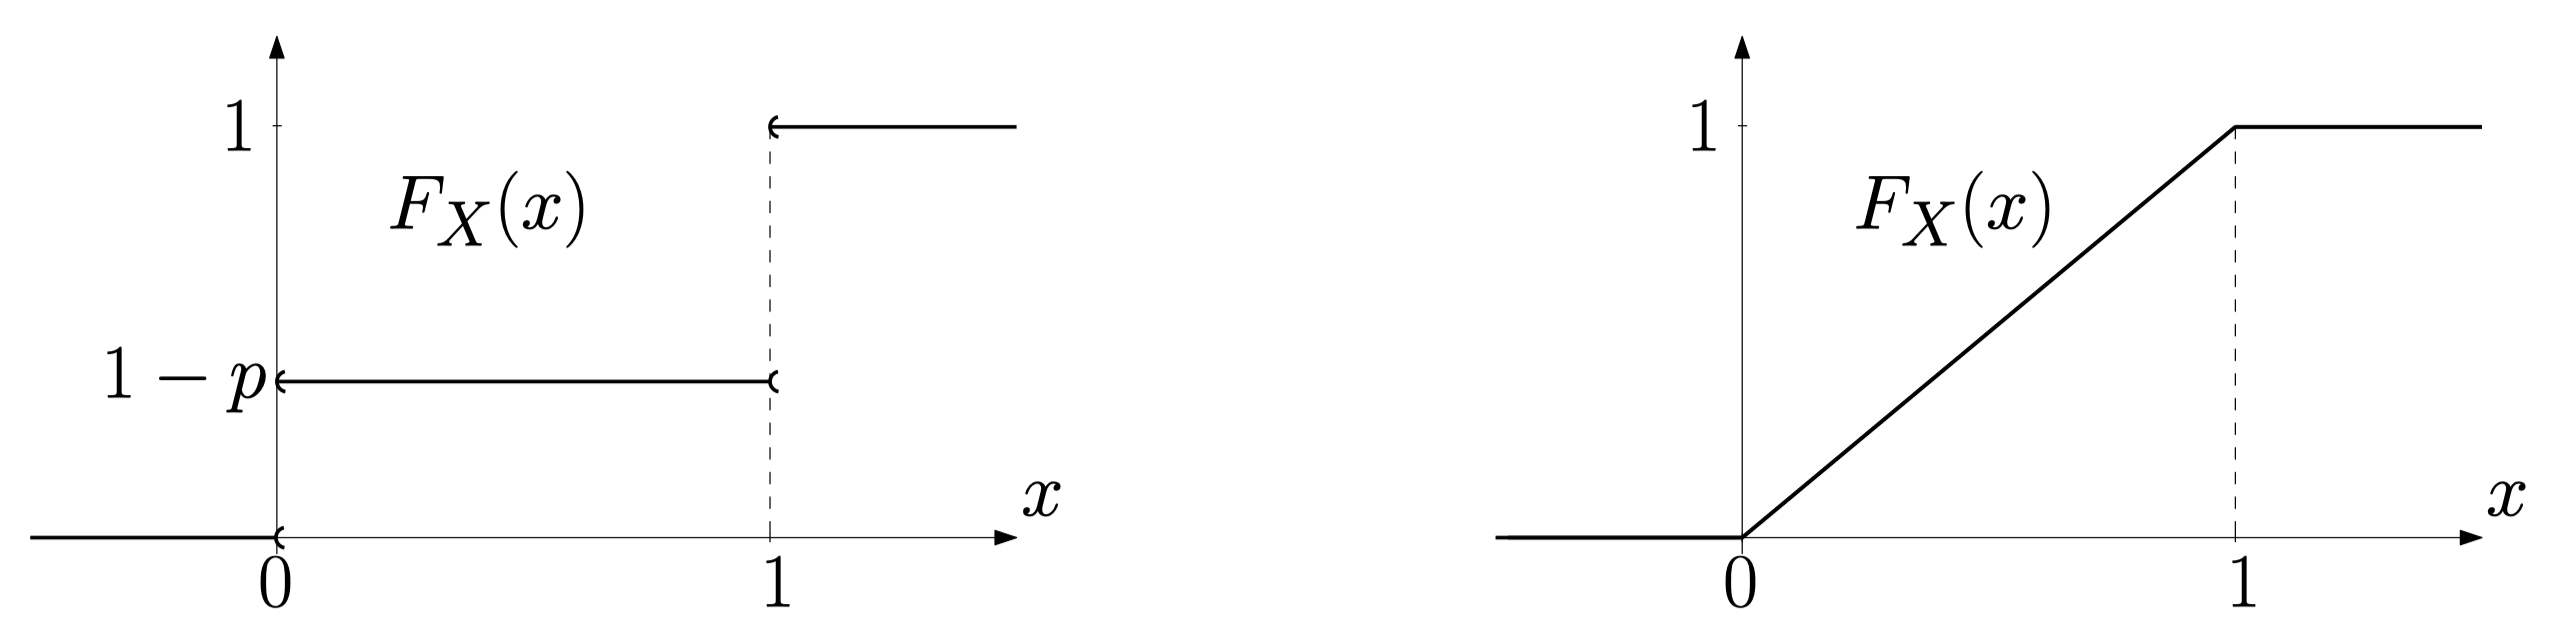
\includegraphics[width=15cm]{../images/WuS_Fig3-1}
    \centering
\end{figure}

Let \(X_1, \, X_2,...\) be a sequence of independent Bernoulli random variables with parameter \(\frac{1}{2}\). For every fixed \(\omega\), we have \(X_1(\omega), \, X_2(\omega),... \in \{0, \, 1\}\). Hence the infinite series
\[
    Y(\omega) = \sum_{n = 1}^{\infty}2^{-n}X_n(\omega)
\]
is absolutely convergent, and we have \(Y(\omega) \in [0, \, 1]\).

\begin{tbox}
    \textbf{Proposition:} The mapping \(Y : \Omega \to [0, \, 1]\) defined by the equation above is a uniform random variable in \([0, \, 1]\).
\end{tbox}

\paragraph{Step 3: Construction of a random variable with an arbitrary distribution \(F\)}

Let \(F : \mathbb{R} \to [0, \, 1]\) satisfying item \((1) - (3)\) at the beginning of the section. If \(F\) is strictly increasing and continuous then \(F\) is one-to-one and one can define its inverse \(F^{-1}\). For every \(\alpha \in [0, \, 1], \, F^{-1}(\alpha)\) is the unique real number \(x\) such that \(F(x) = \alpha\). In such a case, the defines the inverse distribution function. More generally, we can define a generalized inverse for \(F\).

\textbf{Definition (Generalized inverse):} The generalized inverse of \(F\) is the mapping \(F^{-1} : (0, \, 1) \to \mathbb{R}\) defined by
\[
    \forall \alpha \in (0, \, 1) : F^{-1}(\alpha) = \inf\{x \in \mathbb{R} : F(x) \geq \alpha\}.
\]

By definition of the infimum and using right continuity of \(F\), we have for every \(x \in \mathbb{R}\) and \(\alpha \in (0, \, 1)\)
\[
    (F^{-1}(\alpha) \leq x) \iff (\alpha \leq F(x)).
\]

\begin{tbox}
    \textbf{Theorem (inverse transform sampling):} Let \(F : \mathbb{R} \to [0, \, 1]\) satisfying items \((1)-(3)\) at the beginning of the section. Let \(U\) be a uniform random variable in \([0, \, 1]\). Then the random variable
    \[
        X = F^{-1}(U)
    \]
    has distribution \(F_X = F\).
\end{tbox}

\paragraph{Step 4: General sequence of independent random variables}
Finally, we introduce the following theorem:

\begin{tbox}
    Let \(F_1, \, F_2,...\) be a sequence of functions \(\mathbb{R} \to [0, \, 1]\) satisfying items \((1)-(3)\) at the beginning of the section. Then there exists a probability space \((\Omega, \, \mathcal{F}. \, \mathbb{P})\) and a sequence of independent random variables \(X_1, \, X_2,...\) on this probability space such that
    \begin{itemize}
        \item for every \(i \, X_i\) has a distribution function \(F_i\) (i.e. \(\forall x \mathbb{P}[X_i \leq x] = F_i(x)\)), and
        \item \(X_1, \, X_2,...\) are independent.
    \end{itemize}
\end{tbox}

\end{document}